% tikz_hexloop.tex -- Proposition 2.28, the closed curve of contact cells of volume 8.
%   (a) The plane P: the hexagon of roots turned by theta (solid) from its position at theta = 0
%       (dotted), the hexagon Hex_theta of inradius 1 cut out by the six turned roots, the
%       P-directions of the other eighteen roots (the triangles T_+ at 30, 150, 270 degrees and
%       T_- at 90, 210, 330 degrees), and the sector between the rays at 30 and 90 degrees split
%       into the two triangles over which J_1 and J_2 are integrated; C = cos(pi/6 - theta).
%   (b) The slice over a point p of Hex_theta: the two opposite triangles of inradii h_+ and h_-
%       in P', whose intersection is a hexagon when h_+ <= 2 h_- and h_- <= 2 h_+.
%   (c) The cell as the union of its slices: Hex_theta in P, with the slice over three points
%       drawn transversally (a schematic; P' is two-dimensional).
%   (d) Along the curve: sin psi = 4C/(4C^2+3) and the largest inner product 4C^2/(4C^2+3),
%       against theta; both return to their values at the root system at theta = pi/3.
% Build:  pdflatex tikz_hexloop.tex && pdftoppm -r 500 -png -singlefile tikz_hexloop.pdf ../figures/fig_tikz_hexloop
% Test:   python3 tikz_overlap_check.py --auto tikz_hexloop.tex
\documentclass[border=4pt]{standalone}
\usepackage{tikz}
\usepackage{tikz-3dplot}
\usepackage{pgfplots}
\pgfplotsset{compat=1.17}
\usetikzlibrary{positioning,arrows.meta,calc,decorations.markings}
\usepackage[T1]{fontenc}
\usepackage{lmodern}
\usepackage{amsmath,amssymb}
\definecolor{cblue}{HTML}{2A78D6}
\definecolor{corange}{HTML}{EB6834}
\definecolor{caqua}{HTML}{1BAF7A}
\definecolor{cviolet}{HTML}{7A5AC8}
\definecolor{cink}{HTML}{2B2A28}
\definecolor{cink2}{HTML}{52514E}
\definecolor{cink3}{HTML}{8B8A85}
% tikzcheck.tex -- the hooks of tikz_overlap_check.py, input by the TikZ figures.
% Two ways to name what is checked.
%  - Explicit: \figboxes and \figlabels list named nodes; with \nolabels defined,
%    nodes in the style lbl are drawn invisibly.
%  - Automatic: \autocheck in the preamble gives every node of the picture,
%    pgfplots tick labels included, an alias chk<n>; with \nolabels defined, the
%    text of every node is drawn invisibly and its shape is kept.
% \checkfigure, at the end of the picture, writes the four corners of each
% checked node (so that rotated nodes are measured by their true extent) and
% those of the picture to the log when \checkbboxes is defined.
\tikzset{lbl/.style={}}
\ifdefined\nolabels\tikzset{lbl/.append style={opacity=0}}\fi
\newcount\chknodes
\newcommand\autocheck{% idempotent: a figure with \autocheck may also be run with --auto
  \ifdefined\chkauto\else
  \def\chkauto{}%
  \tikzset{every node/.append style={/utils/exec={\global\advance\chknodes by 1\relax},
                                      alias=chk\the\chknodes}}%
  \ifdefined\nolabels\tikzset{every node/.append style={text opacity=0}}\fi
  \fi}
\makeatletter
% a node counted but never kept (pgfplots typesets some nodes once to measure them)
% has no shape, and is skipped
\newcommand\chkifnode[2]{\pgfutil@ifundefined{pgf@sh@ns@#1}{}{#2}}
\makeatother
\newcommand\chkout[2]{% kind, node
  \path let \p1=(#2.south west), \p2=(#2.north east), \p3=(#2.north west), \p4=(#2.south east)
    in \pgfextra{\typeout{BBOX #1 #2\space\x1\space\y1\space\x2\space\y2\space\x3\space\y3\space\x4\space\y4}};}
\newcommand\checkfigure{%
  \ifdefined\checkbboxes
    \path let \p1=(current bounding box.south west), \p2=(current bounding box.north east)
      in \pgfextra{\typeout{PICBB \x1\space\y1\space\x2\space\y2}};
    \typeout{BORDER 4.0pt}%
    \ifdefined\chkauto
      \edef\chklast{\the\chknodes}%
      \foreach \nm in {1,...,\chklast} {\chkifnode{chk\nm}{\chkout{auto}{chk\nm}}}%
    \else
      \foreach \nm in \figboxes {\chkout{box}{\nm}}%
      \foreach \nm in \figlabels {\chkout{label}{\nm}}%
    \fi
  \fi}
\ifdefined\forceauto\autocheck\fi

\autocheck
\begin{document}
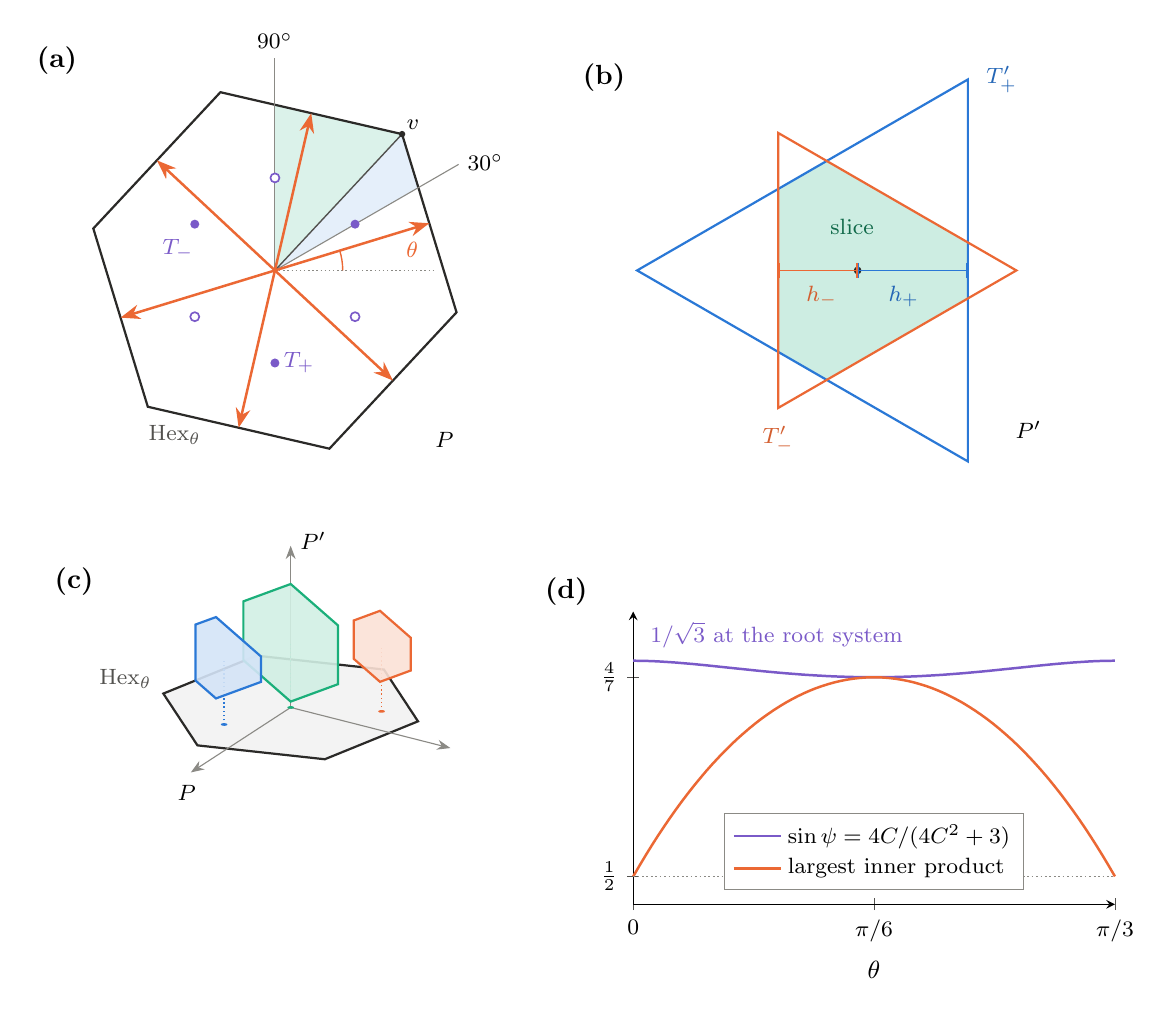
\begin{tikzpicture}[font=\small, >=Stealth]
%% ------------------------------------------------------------------ (a) the plane P
\def\th{17}          % theta in degrees, for the drawing
\pgfmathsetmacro\C{cos(30-\th)}
\begin{scope}[scale=2.05]
  % sector between 30 and 90 degrees, split into its two triangles
  \coordinate (O) at (0,0);
  \coordinate (B1) at ({cos(30)/\C},{sin(30)/\C});
  \coordinate (B2) at ({cos(90)/\C},{sin(90)/\C});
  \coordinate (V) at ({2/sqrt(3)*cos(\th+30)},{2/sqrt(3)*sin(\th+30)});
  \fill[cblue!12] (O) -- (B1) -- (V) -- cycle;
  \fill[caqua!16] (O) -- (V) -- (B2) -- cycle;
  % Hex_theta: edge normals e(theta + 60 m), inradius 1, vertices at radius 2/sqrt3
  \draw[cink, line width=0.8pt] ({2/sqrt(3)*cos(\th+30)},{2/sqrt(3)*sin(\th+30)})
    \foreach \m in {1,...,5} { -- ({2/sqrt(3)*cos(\th+30+60*\m)},{2/sqrt(3)*sin(\th+30+60*\m)}) } -- cycle;
  % the rays at 30 and 90 degrees
  \draw[cink3, line width=0.4pt] (O) -- ($(O)!1.28!(B1)$);
  \draw[cink3, line width=0.4pt] (O) -- ($(O)!1.28!(B2)$);
  \draw[cink2, line width=0.5pt] (O) -- (V);
  % hexagon of roots at theta = 0 (dotted) and turned by theta (solid)
  \draw[cink3, densely dotted, line width=0.5pt] (O) -- (1,0);
  \foreach \m in {0,...,5} {
    \draw[corange, line width=0.9pt, ->] (O) -- ({cos(\th+60*\m)},{sin(\th+60*\m)});
  }
  % theta arc between e(0) and e(theta)
  \draw[corange, line width=0.5pt] (0.42,0) arc (0:\th:0.42);
  \node[text=corange, font=\footnotesize] at ({0.86*cos(\th/2)},{0.86*sin(\th/2)}) {$\theta$};
  % P-directions of the other eighteen roots: T_+ (filled) and T_- (open), at radius sigma
  \pgfmathsetmacro\sg{4*\C/(4*\C*\C+3)}
  \foreach \a in {30,150,270} \fill[cviolet] ({\sg*cos(\a)},{\sg*sin(\a)}) circle (0.028);
  \foreach \a in {90,210,330} \draw[cviolet, fill=white, line width=0.6pt] ({\sg*cos(\a)},{\sg*sin(\a)}) circle (0.028);
  % labels
  \fill[cink] (V) circle (0.02);
  \node[anchor=south west, inner sep=1.5pt, font=\footnotesize] at (V) {$v$};
  \node[anchor=west, inner sep=2pt, font=\footnotesize] at ($(O)!1.30!(B1)$) {$30^\circ$};
  \node[anchor=south, inner sep=2pt, font=\footnotesize] at ($(O)!1.30!(B2)$) {$90^\circ$};
  \node[font=\footnotesize, text=cink2] at (-0.62,-1.02) {$\mathrm{Hex}_\theta$};
  \node[font=\footnotesize, text=cviolet] at (0.15,-0.57) {$T_+$};
  \node[font=\footnotesize, text=cviolet] at (-0.60,0.13) {$T_-$};
  \node[font=\bfseries] at (-1.35,1.30) {(a)};
  \node[font=\footnotesize] at (1.05,-1.05) {$P$};
\end{scope}
%% ------------------------------------------------------------------ (b) the slice in P'
\begin{scope}[xshift=7.4cm, scale=1.40]
  \def\hp{1.00}\def\hm{0.72}
  % T_+ : normals at 0, 120, 240, inradius hp; vertices at 2 hp opposite the normals
  \coordinate (P1) at ({2*\hp*cos(180)},{2*\hp*sin(180)});
  \coordinate (P2) at ({2*\hp*cos(300)},{2*\hp*sin(300)});
  \coordinate (P3) at ({2*\hp*cos(60)},{2*\hp*sin(60)});
  \coordinate (M1) at ({2*\hm*cos(0)},{2*\hm*sin(0)});
  \coordinate (M2) at ({2*\hm*cos(120)},{2*\hm*sin(120)});
  \coordinate (M3) at ({2*\hm*cos(240)},{2*\hm*sin(240)});
  \begin{scope}
    \clip (P1) -- (P2) -- (P3) -- cycle;
    \fill[caqua!22] (M1) -- (M2) -- (M3) -- cycle;
  \end{scope}
  \draw[cblue, line width=0.8pt] (P1) -- (P2) -- (P3) -- cycle;
  \draw[corange, line width=0.8pt] (M1) -- (M2) -- (M3) -- cycle;
  \fill[cink] (0,0) circle (0.035);
  % inradii
  \draw[cblue, line width=0.6pt, |-|] (0,0) -- ({\hp*cos(0)},{\hp*sin(0)});
  \draw[corange, line width=0.6pt, |-|] (0,0) -- ({\hm*cos(180)},{\hm*sin(180)});
  \node[text=cblue!85!black, font=\footnotesize, anchor=north] at ({0.42*\hp},-0.05) {$h_+$};
  \node[text=corange!90!black, font=\footnotesize, anchor=north] at ({-0.45*\hm},-0.05) {$h_-$};
  \node[text=cblue!85!black, font=\footnotesize, anchor=west] at ($(P3)+(0.08,0)$) {$T_+'$};
  \node[text=corange!90!black, font=\footnotesize, anchor=north] at ($(M3)+(0,-0.08)$) {$T_-'$};
  \node[font=\footnotesize, text=caqua!60!black] at (-0.05,0.40) {slice};
  \node[font=\bfseries] at (-2.30,1.75) {(b)};
  \node[font=\footnotesize] at (1.55,-1.45) {$P'$};
\end{scope}
%% ------------------------------------------------------------------ (c) the union of the slices
%% slices computed at theta = 17 degrees, sigma = 0.5734: over p_1 = 0 (h_+ = h_- = 1.221),
%% p_2 = (0.62, -0.30) (h_+ = 0.950, h_- = 0.740) and p_3 = (-0.35, 0.72) (h_+ = 0.756, h_- = 0.717)
\tdplotsetmaincoords{66}{122}
\begin{scope}[shift={(0.2,-5.55)}, tdplot_main_coords, scale=1.45]
  \draw[cink, line width=0.8pt, fill=cink3!10] ({2/sqrt(3)*cos(47)},{2/sqrt(3)*sin(47)},0)
    \foreach \m in {1,...,5} { -- ({2/sqrt(3)*cos(47+60*\m)},{2/sqrt(3)*sin(47+60*\m)},0) } -- cycle;
  \draw[cink3, ->, line width=0.4pt] (0,0,0) -- (1.65,0,0);
  \draw[cink3, ->, line width=0.4pt] (0,0,0) -- (0,1.65,0);
  \draw[cink3, ->, line width=0.4pt] (0,0,0) -- (0,0,1.55);
  \def\sc{0.40}
  \foreach \px/\py/\col/\pts in {
      0/0/caqua/{(-1.221,-0.705),(0.000,-1.409),(1.221,-0.705),(1.221,0.705),(0.000,1.409),(-1.221,0.705)},
      0.62/-0.30/cblue/{(-0.740,-0.670),(-0.210,-0.975),(0.950,-0.306),(0.950,0.306),(-0.210,0.975),(-0.740,0.670)},
      -0.35/0.72/corange/{(-0.717,-0.460),(-0.040,-0.851),(0.756,-0.391),(0.756,0.391),(-0.040,0.851),(-0.717,0.460)}} {
    \fill[\col] (\px,\py,0) circle (0.03);
    \draw[\col, line width=0.5pt, densely dotted] (\px,\py,0) -- (\px,\py,0.62);
  }
  \foreach \px/\py/\col/\pts in {
      0/0/caqua/{-1.221/-0.705,0.000/-1.409,1.221/-0.705,1.221/0.705,0.000/1.409,-1.221/0.705},
      0.62/-0.30/cblue/{-0.740/-0.670,-0.210/-0.975,0.950/-0.306,0.950/0.306,-0.210/0.975,-0.740/0.670},
      -0.35/0.72/corange/{-0.717/-0.460,-0.040/-0.851,0.756/-0.391,0.756/0.391,-0.040/0.851,-0.717/0.460}} {
    \draw[\col, line width=0.8pt, fill=\col!20, fill opacity=0.9]
      \foreach \u/\w [count=\i] in \pts { \ifnum\i=1 (\px,{\py+\sc*\u},{0.62+\sc*\w}) \else -- (\px,{\py+\sc*\u},{0.62+\sc*\w}) \fi } -- cycle;
  }
  \node[font=\footnotesize, anchor=north] at (1.72,0,0) {$P$};
  \node[font=\footnotesize, anchor=west] at (0,0,1.60) {$P'$};
  \node[font=\footnotesize, text=cink2] at (0.25,-1.55,0) {$\mathrm{Hex}_\theta$};
\end{scope}
\node[font=\bfseries] at (-2.55,-3.95) {(c)};
%% ------------------------------------------------------------------ (d) along the curve
\begin{axis}[name=D, at={(4.55cm,-8.05cm)}, anchor=south west, width=7.7cm, height=5.3cm,
    xmin=0, xmax=1.0472, ymin=0.49, ymax=0.595,
    xtick={0,0.5236,1.0472}, xticklabels={$0$,$\pi/6$,$\pi/3$},
    ytick={0.5,0.5714}, yticklabels={$\tfrac12$,$\tfrac47$},
    xlabel={$\theta$}, axis lines=left, tick style={cink2}, tick label style={font=\footnotesize},
    legend cell align=left, legend style={font=\footnotesize, at={(0.5,0.05)}, anchor=south, draw=cink3, fill=white},
    clip=false]
  \addplot[cviolet, line width=0.9pt, domain=0:1.0472, samples=80] {4*cos(deg(pi/6-x))/(4*cos(deg(pi/6-x))^2+3)};
  \addlegendentry{$\sin\psi=4C/(4C^2+3)$}
  \addplot[corange, line width=0.9pt, domain=0:1.0472, samples=80] {4*cos(deg(pi/6-x))^2/(4*cos(deg(pi/6-x))^2+3)};
  \addlegendentry{largest inner product}
  \addplot[cink3, densely dotted, line width=0.6pt, domain=0:1.0472] {0.5};
  \coordinate (Dq) at (axis cs:0.03,0.5774);
\end{axis}
\node[font=\footnotesize, text=cviolet, anchor=south west, inner sep=1pt] at ($(Dq)+(0,0.12)$) {$1/\sqrt3$ at the root system};
\node[font=\bfseries] at ($(D.north west)+(-0.85cm,0.25cm)$) {(d)};
\checkfigure
\end{tikzpicture}
\end{document}
